\chapter{Graphical User Interface}
\label{user-gui}

Running \textttuse{ivette} displays the
\FramaC Graphical User Interface (GUI), Ivette ({\em Integrated Verification
  Environment Toolkit for Trusted Execution}).

Ivette is based on the Electron\footnote{\url{https://www.electronjs.org/}}
framework and is thus not always directly distributed with \FramaC,
especially if you installed it using your distribution's package manager.

For an Opam-based installation of \FramaC, running \textttuse{ivette} for the
first time will trigger a script that downloads, compiles, installs and runs
Ivette. This script requires some tools such as Node.js and Yarn.
Subsequent executions of \textttuse{ivette} will directly run the installed
executable.

Note that Ivette is also distributed as a standalone executable in the \FramaC
website, as AppImage on Linux and Apple Disk Image (.dmg) on macOS.

\begin{figure}[htbp]
\begin{center}
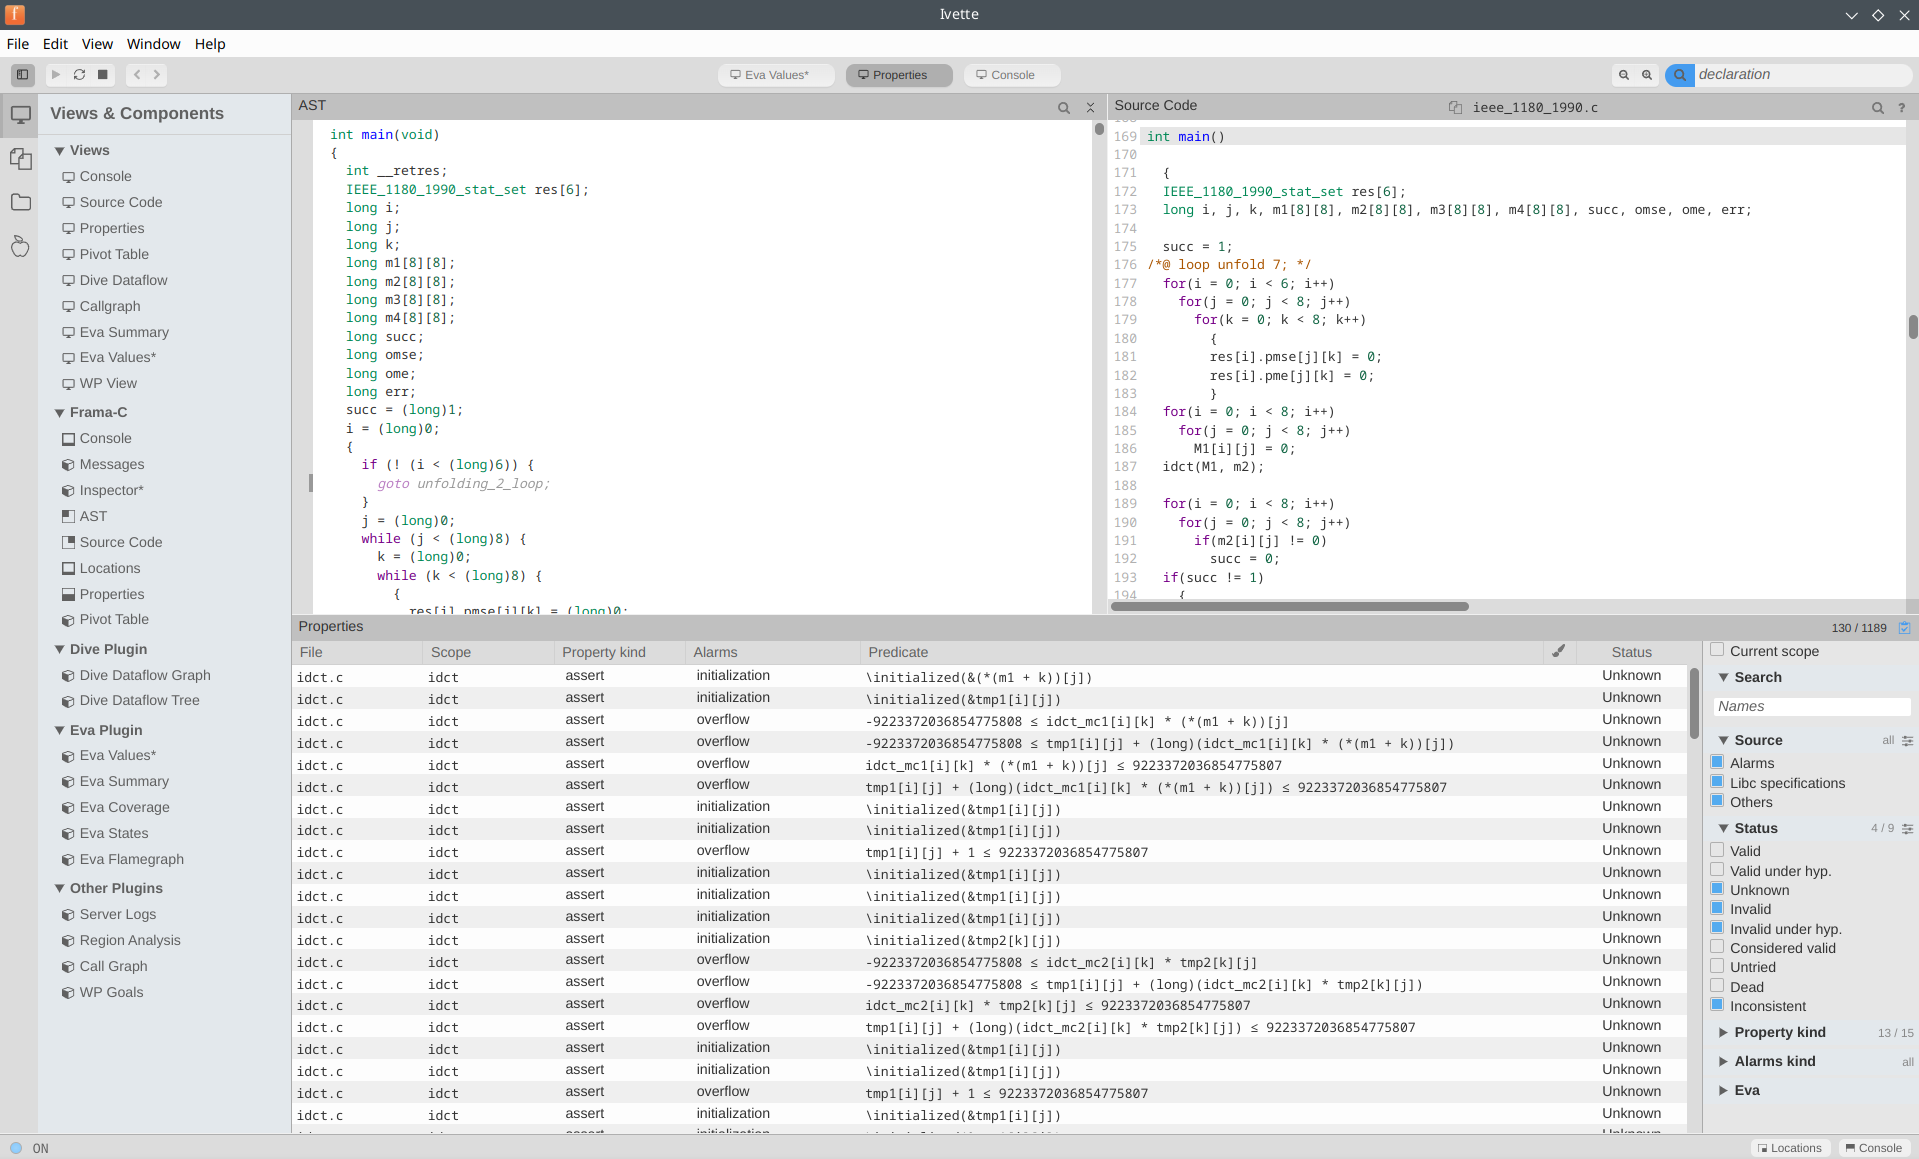
\includegraphics[width=0.95\textwidth]{ivette.png}
\end{center}
\caption{Screenshot of Ivette, illustrating several components}
\label{fig:ivette}
\end{figure}

Ivette's documentation is accessible from its interface, via the
{\em Help - Documentation} menu, and from each component's question mark (?)
button. Clicking on them opens a dialog with the relevant documentation.

\section{Command-line options}

\textttuse{ivette} accepts almost all command-line options that
\texttt{frama-c} does, so you can usually replace \texttt{frama-c <options>}
with \texttt{ivette <options>} to run an analysis and see its results.

There are currently a few options that are intercepted by the
Electron process itself instead of passed on to the underlying \texttt{frama-c}
process:

\begin{itemize}
\item \texttt{-{}-no-sandbox}: this option avoids issues with Electron
  sandboxing (with e.g. Ubuntu 24.04).
  {\em Note that this may have security implications.}
\item \texttt{-{}-settings <file.json|CLEAN>}: allows using a specific settings
  file. The special value \texttt{CLEAN} launches Ivette with default settings.
\item \texttt{-{}-working <dir>}: uses \texttt{<dir>} as working directory.
\end{itemize}
